\documentclass[informe.tex]{subfiles}
\begin{document}


\textbf{Función de transformación}\newline

La función de transformación de un filtro pasa banda (BP) no normalizado, $T_{BP}(s)$, hacia un filtro pasa bajo normalizado (LP), $T_{LP}(S)$, es:
	
	\begin{equation}
		\label{eqn:bp:lp1}	
		S=\frac{s^2 + \omega_0^2}{B \cdot s}
	\end{equation}
	
o bien
	
	\begin{equation}
		\label{eqn:bp:lp2}	
		\Omega = \frac{ \omega^2 - \omega_0^2}{B \cdot \omega}	
	\end{equation}
		
donde,
	
	\begin{tabbing}
		$B=|\omega_{x} - \omega_{-x}|$, es el ancho de banda de paso del filtro. \\
		$\omega_0^2=\omega_1 \cdot \omega_2 =\omega_3 \cdot \omega_4 $, es la frecuencia central (media geométrica) del filtro pasa banda.
	\end{tabbing}

		
\textbf{\newline Procedimiento de resolución de filtros pasa banda}\newline

	1-Al conjunto de requerimientos de un filtro pasa banda:
	\begin{center}			 
				($A_{max}$, $\omega_1$, $\omega_2$, $A_{min}$, $\omega_3$, $\omega_4$)
	\end{center}
se transforman con la función dada en la Ec. \ref{eqn:bp:lp2} a los requerimientos equivalentes del filtro paso bajo normalizado (LP), quedando que
    \begin{center}
				($A_{max}$, $\Omega_P=1$, $A_{min}$, 
				  $\Omega_S=\frac{\omega_2 - \omega_1}
				                 {\omega_4 - \omega_3}
				  $)
    \end{center}				
	
	\begin{figure}[h]
		\centering
		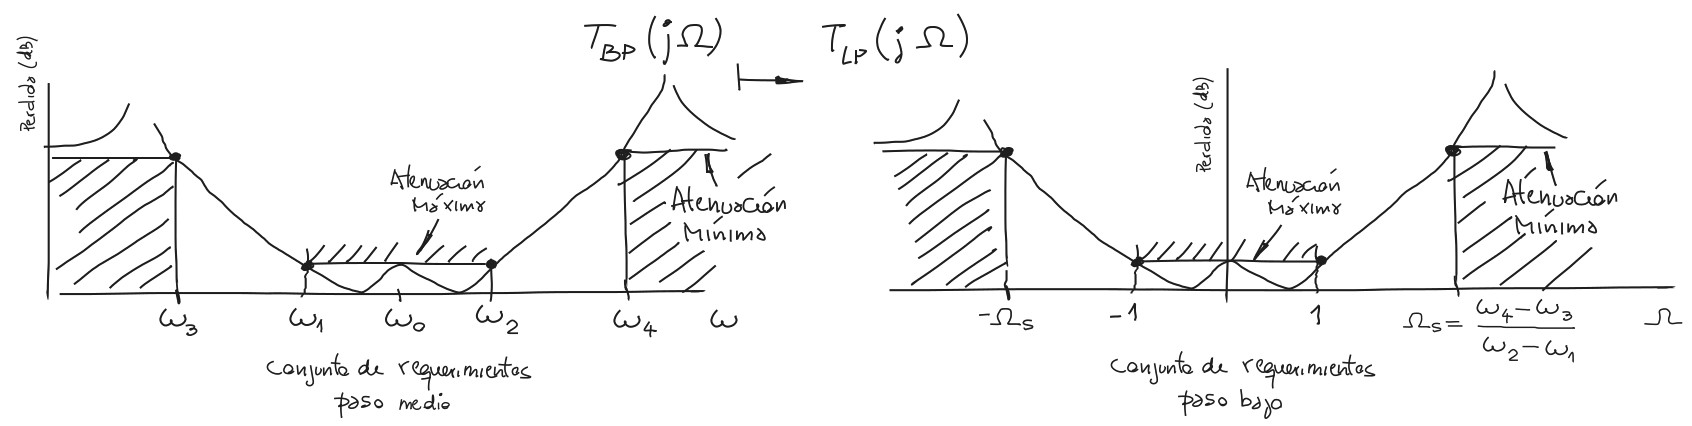
\includegraphics[scale=1.2]{transformacion_4_bp.jpg}
		\caption{Funciones de atenuación. A la izquierda el filtro pasa banda. A la derecha el filtro pasa bajo normalizado}
		\label{fig:transformacion:bp:func_att}
	\end{figure}	
		
	\begin{figure}[h]
		\centering
		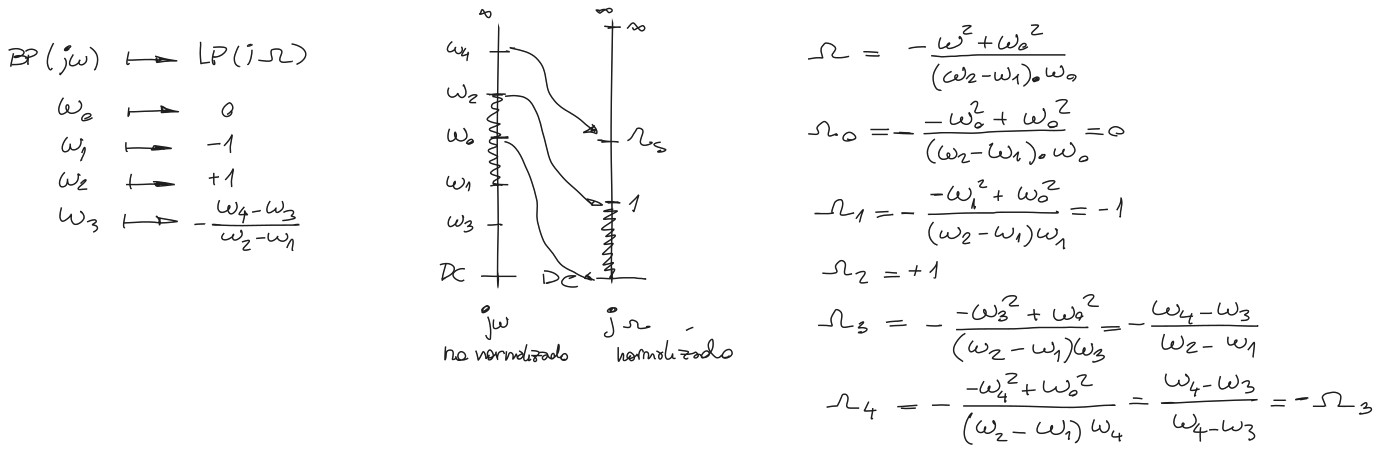
\includegraphics[scale=1.3]{transformacion_5_bp.jpg}
		\caption{Relaciones entre las frecuencias de un filtro pasa banda y un filtro pasa bajo normalizado}
		\label{fig:transformacion:bp:relaciones}
	\end{figure}		

	2- Seguido, se determina la función que aproxime los requerimientos pasa bajos según la aplicación (Butterworth, Chebyshev o Bessel).	
	
	3- Por último, la función $T_{LP}(S)$ se transforma a la función $T_{BP}(s)$ talque 
				$$T_{BP}(s)= \left. T_{LP}(S) \right|_{S=(s^2+\omega^2_0)/B}$$
				
%%  
\textbf{Ejemplo con Matlab:} Filtro chebyshev pasa medio - diseño por transformación de frecuencia, Fig. \ref{fig:transformacion:bp:ej1_freqs_bp}.\newline  

\lstinputlisting[language=Matlab, frame=single, extendedchars=true]{./src_matlab/mi_lp2bp.m}  		

\lstinputlisting[language=Matlab, frame=single, extendedchars=true]{./src_matlab/lp2bp_ej1_chebyshev.m} 

\begin{figure}[h]
     \centering
     \begin{subfigure}[b]{0.3\textwidth}
         \centering
         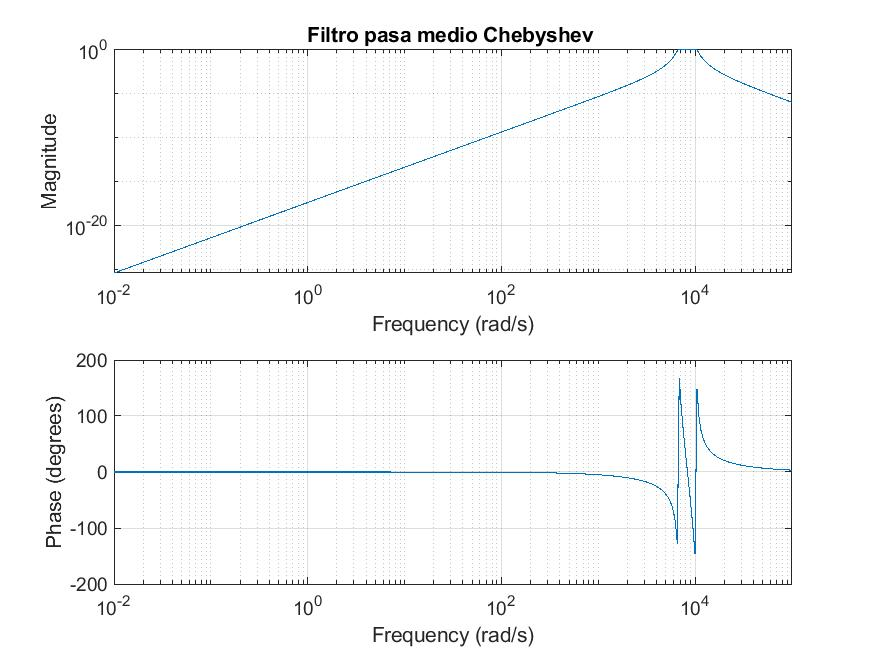
\includegraphics[scale=0.2]{lp2bp_ej1_chebyshev_freqs}
         \caption{Respuesta en frecuencia, filtro pasa banda de Chebyshev}
         \label{fig:transformacion:bp:ej1_freqs_bp:freqs_bp}
     \end{subfigure}
     \hfill
     \begin{subfigure}[b]{0.3\textwidth}
         \centering
         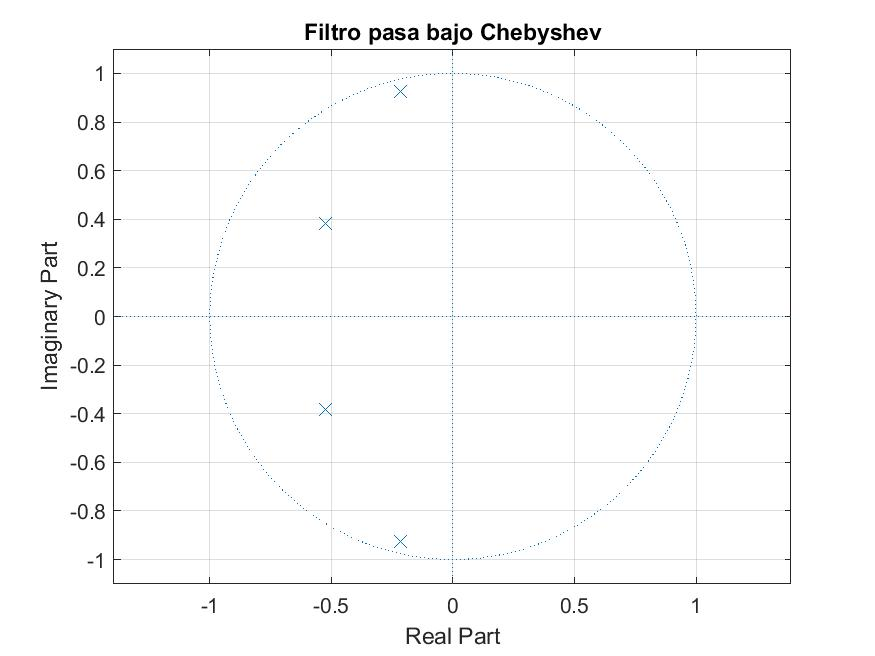
\includegraphics[scale=0.2]{lp2bp_ej1_chebyshev_pz_lp.jpg}
         \caption{Diagrama de polos y ceros, filtro pasa bajo normalizado de Chebyshev}
         \label{fig:transformacion:bp:ej1_freqs_lp:pz}
     \end{subfigure}
     \hfill
     \begin{subfigure}[b]{0.3\textwidth}
         \centering
         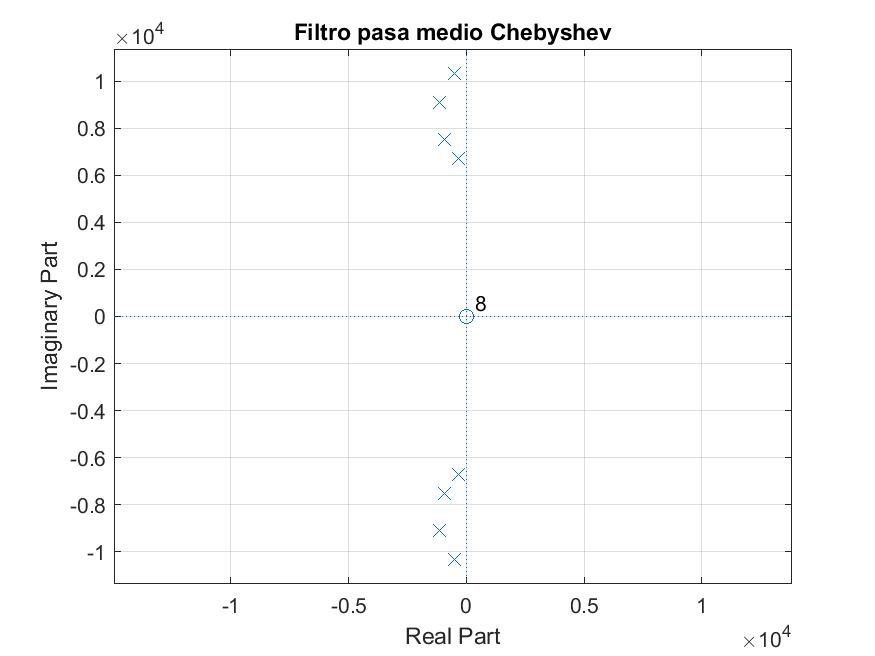
\includegraphics[scale=0.2]{lp2bp_ej1_chebyshev_pz_bp.jpg}
         \caption{Diagrama de polos y ceros, filtro pasa banda de Chebyshev}
         \label{fig:transformacion:bp:ej1_freqs_bp:pz}
     \end{subfigure}
 	 \caption{Ejemplo 1. Filtro pasa banda de Chebyshev}
     \label{fig:transformacion:bp:ej1_freqs_bp}
\end{figure}


\end{document}	